\section{Object Holding (Jakub Jędrzejczyk)}

For the sake of manipulating holdable objects within 3D space an actor blueprint called \lstinline[language=C]|Hand| was created.

The hand is represented visually by a simple sphere mesh, as seen in figure \ref{fig:HandBlueprint}.
It also includes a spline, which was planned to be used for interacting with virtual user interfaces, for example for user settings.
The red arrow seen in the figure represents the forward vector of the hand, and is seen in debug view (e.g. within the editor), but not in the final application.
As no directly interactive interfaces were implemented, this functionality was disabled in the final product.

\begin{figure}[H]
	\centering
		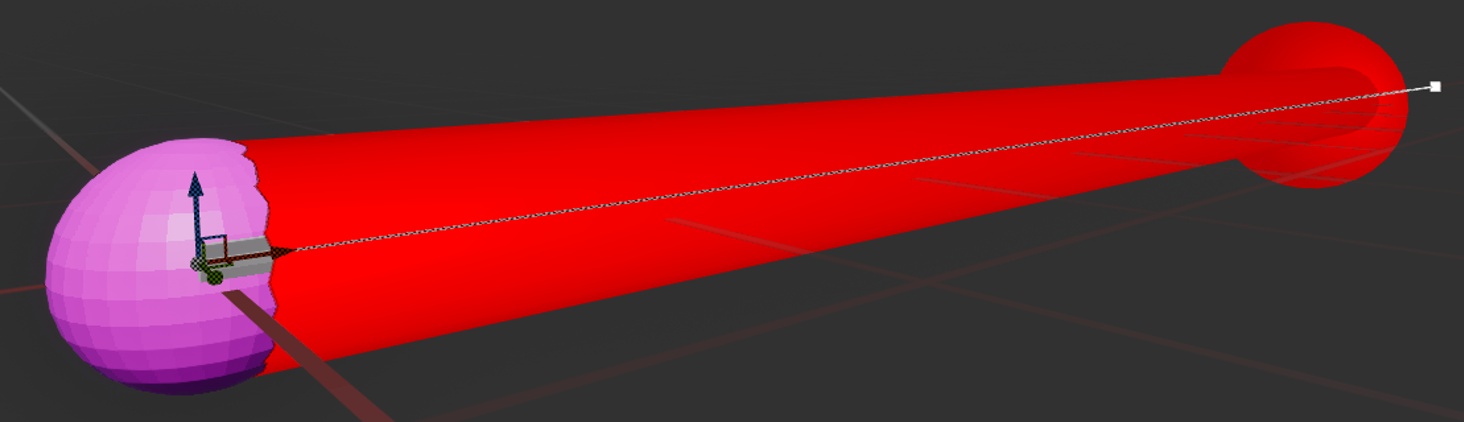
\includegraphics[width=0.8\textwidth]{Images/HandObject.png}
	\caption{Hand blueprint within the editor.}
	\label{fig:HandBlueprint}
\end{figure}

The hand's default color is pink, but this can be easily changed as the object's initialization includes modifying the material of the mesh and saving the reference to its material instance.
The hand also exposes a function called \lstinline[language=C]|SetColor()|, which allows for changing the hand's color at runtime.

While the previously described \lstinline[language=C]|Hand| blueprint represents a hand's logic, this logic was designed to be independent of which hand it represents.
A limitation, based on the fact that most, if not all, users only have up to two hands, is that the hands are distinguished by the \lstinline[language=C]|isLeft| boolean property.
It is theoretically possible to further generalize this logic, but with the application only expecting one user at a time, this limitation was deemed acceptable.

Thus, additional blueprints called \lstinline[language=C]|LeftHand| and \lstinline[language=C]|RightHand| were created, which inherit from the base \lstinline[language=C]|Hand| class.
Their initialization includes setting the \lstinline[language=C]|isLeft| property accordingly, as well as changing the hand's color to orange for the left hand, and blue for the right hand.

For the sake of discerning the hands, choosing a set of contrasting colors was deemed important.
While research shows that red-green colors generally provide the highest contrast \cite{yaoMeasurementsHumanVision2011}, red and green, particularly in Europe, are often associated with negative and positive actions respectively \cite{grzybowskiWhatColorHow2019}.
To avoid any subconscious associations, the second ranking set of colors, blue and yellow was chosen, though due to the perceived brightness of yellows in the CAVE, the yellow was shifted into a softer orange.

The logic discussed further concerns the base \lstinline[language=C]|Hand| class, and thus applies to both hands.

The hand most notably makes use of the \lstinline[language=C]|OnActorBeginOverlap| and \lstinline[language=C]|OnActorEndOverlap| events to determine when it is in contact with a holdable object.
The hand includes an array of references to all currently overlapping holdable objects, the former of the events adding objects to it, and the latter removing them, highlighting one of these objects.

For the sake of intuitiveness, ease of use, and ease of development, the hand only ever highlights one object at a time, prioritizing the smallest one.
Should multiple objects be allowed to be highlighted at once, it would require further testing, on top of being potentially overwhelming and confusing for the user.
This decision is based on the assumption that a smaller object will be more difficult to pick, particularly in a tight environment, which is often encountered when building a PC due to the components' sizes.
Should the user instead mean to pick up a larger object, it should be relatively easy to find a spot where it is not overlapping with any smaller objects.

The highlighting takes after the hand's color, adding a glowing effect to the object using a dynamic material instance.
Originally, the plan was to add an outline effect to the object (see fig. \ref{fig:firsthighlighting}) \cite{unrealuniversityHowHightlightAny2024}, but due to the way it was rendered (adding planes expanded from each side of the object's mesh), this effect required fine-tuning of its arguments to produce visually appealing results for both small and large objects.
This complexity was deemed unnecessary, so the choice was made to instead use a glowing overlay material (see fig. \ref{fig:currenthighlighting}) \cite{unrealartwithalirezaAmazingOverlayHighlight2025}, which only has one downside, of not visually "enlarging" small objects as the outline effect would.
This trade-off was deemed acceptable.

\begin{figure}[H]
	\centering
	\subfigure[]{
		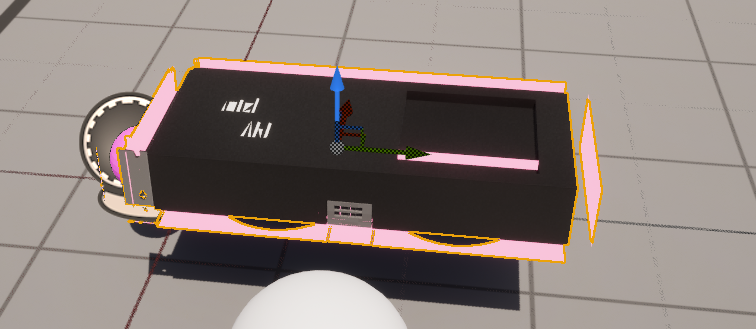
\includegraphics[width=0.45\textwidth]{Images/FirstHighlighting.png}
		\label{fig:firsthighlighting}
	}%
	\hfil
	\subfigure[]{
		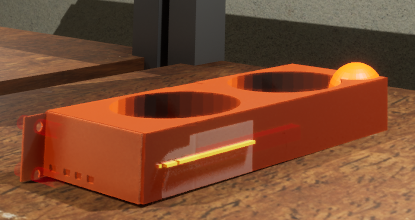
\includegraphics[width=0.45\textwidth]{Images/CurrentHighlighting.png}
		\label{fig:currenthighlighting}
	}
	\caption{Screenshots of the highlighting effect on a holdable object: (a) original outline effect, (b) current glowing effect.}
    \label{fig:highlightingeffects}
\end{figure}

This glow effect makes use of a rounded sine wave to manipulate the intensity of the color being overlaid on the object, producing a smooth pulsing effect.
A standard sine wave is not desired in this instance as it retains its edge values for too short a period of time, making the pulsing feel too abrupt.

The hand also utilizes Unreal Engine's event dispatchers \cites{tylerserinoEventDispatchersUnreal2023}{EventDispatchersUnreal}, allowing other objects to subscribe to the hand's position updates.

\begin{figure}[H]
	\centering
		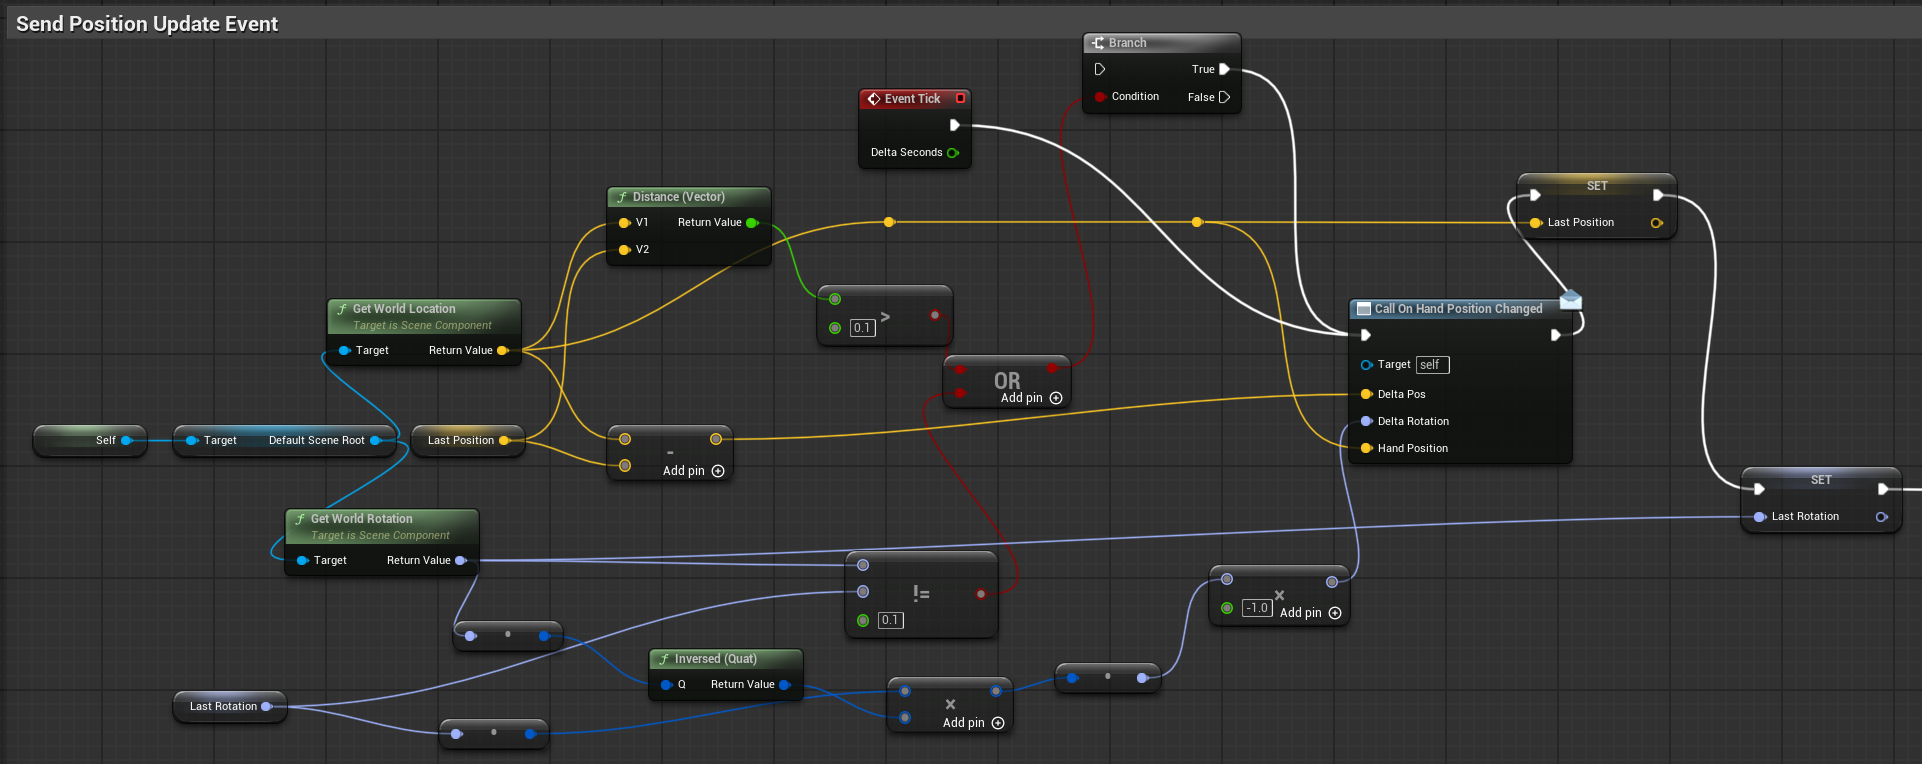
\includegraphics[width=0.95\textwidth]{Images/HandPositionUpdate.png}
	\caption{Blueprints sending events regarding hand position updates.}
	\label{fig:HandPositionUpdate}
\end{figure}

Notable is the requirement of the rotation being converted from Euler angles (pitch, yaw, roll), described within Unreal Engine in the form of a struct called the rotator to a quaternion representation in an effort to avoid an occurrence known as Gimbal lock which happens when two rotation axes become aligned, causing loss of one rotational degree of freedom \cites{diebel2006representing}{diazQuaternionicApproachTeaching2025a}. 
This effectively means that a simple subtraction of two sets of Euler angles may, in some cases, produce incorrect results.
To combat this issue, after being converted to quaternions, the two quaternions are multiplied together, with one of them being conjugated (inverted).
As multiplication of quaternions is not commutative \cite{kuipers1999quaternions}, it's important to note which quaternion is conjugated.
With quaternion multiplication being equal to the composition of rotations \cite{kuipers1999quaternions}, and the latter of the two angles being inverted, the resulting quaternion effectively represents the difference between the two rotations, at which point it is converted back to Euler angles to be stored and used again in the next cycle.

The second hand functionality was disabled in the final product, 